% Niveau :      PCSI *
% Discipline :  Chimie Orga
% Mots clés :  SN, stéréo, cyclohexane

\begin{exercise}{\'Expérience d'Eschenmoser}{3}{PCSI}
{Chimie organique I, SN}{bermu}

\begin{questions}
\questioncours Donnez les mécanismes réactionnels de la $\mathrm{S_N1}$ et de la $\mathrm{S_N2}$ et comparez dans un tableau les différentes propriétés associées (contrôle, sélectivité, nature des réactifs, influence du solvant, de la température, de la concentration ...).

\begin{EnvUplevel}
    En 1970, Albert Eschenmoser réalise une expérience mettant en jeu un réactif $\boldsymbol{\mathrm{(R_H)}}$ et le même réactif avec deux marqueurs deutérés $\mathrm{CD_3}$ $\boldsymbol{\mathrm{(R_D)}}$ en proportion $1:1$,
    \begin{center}
        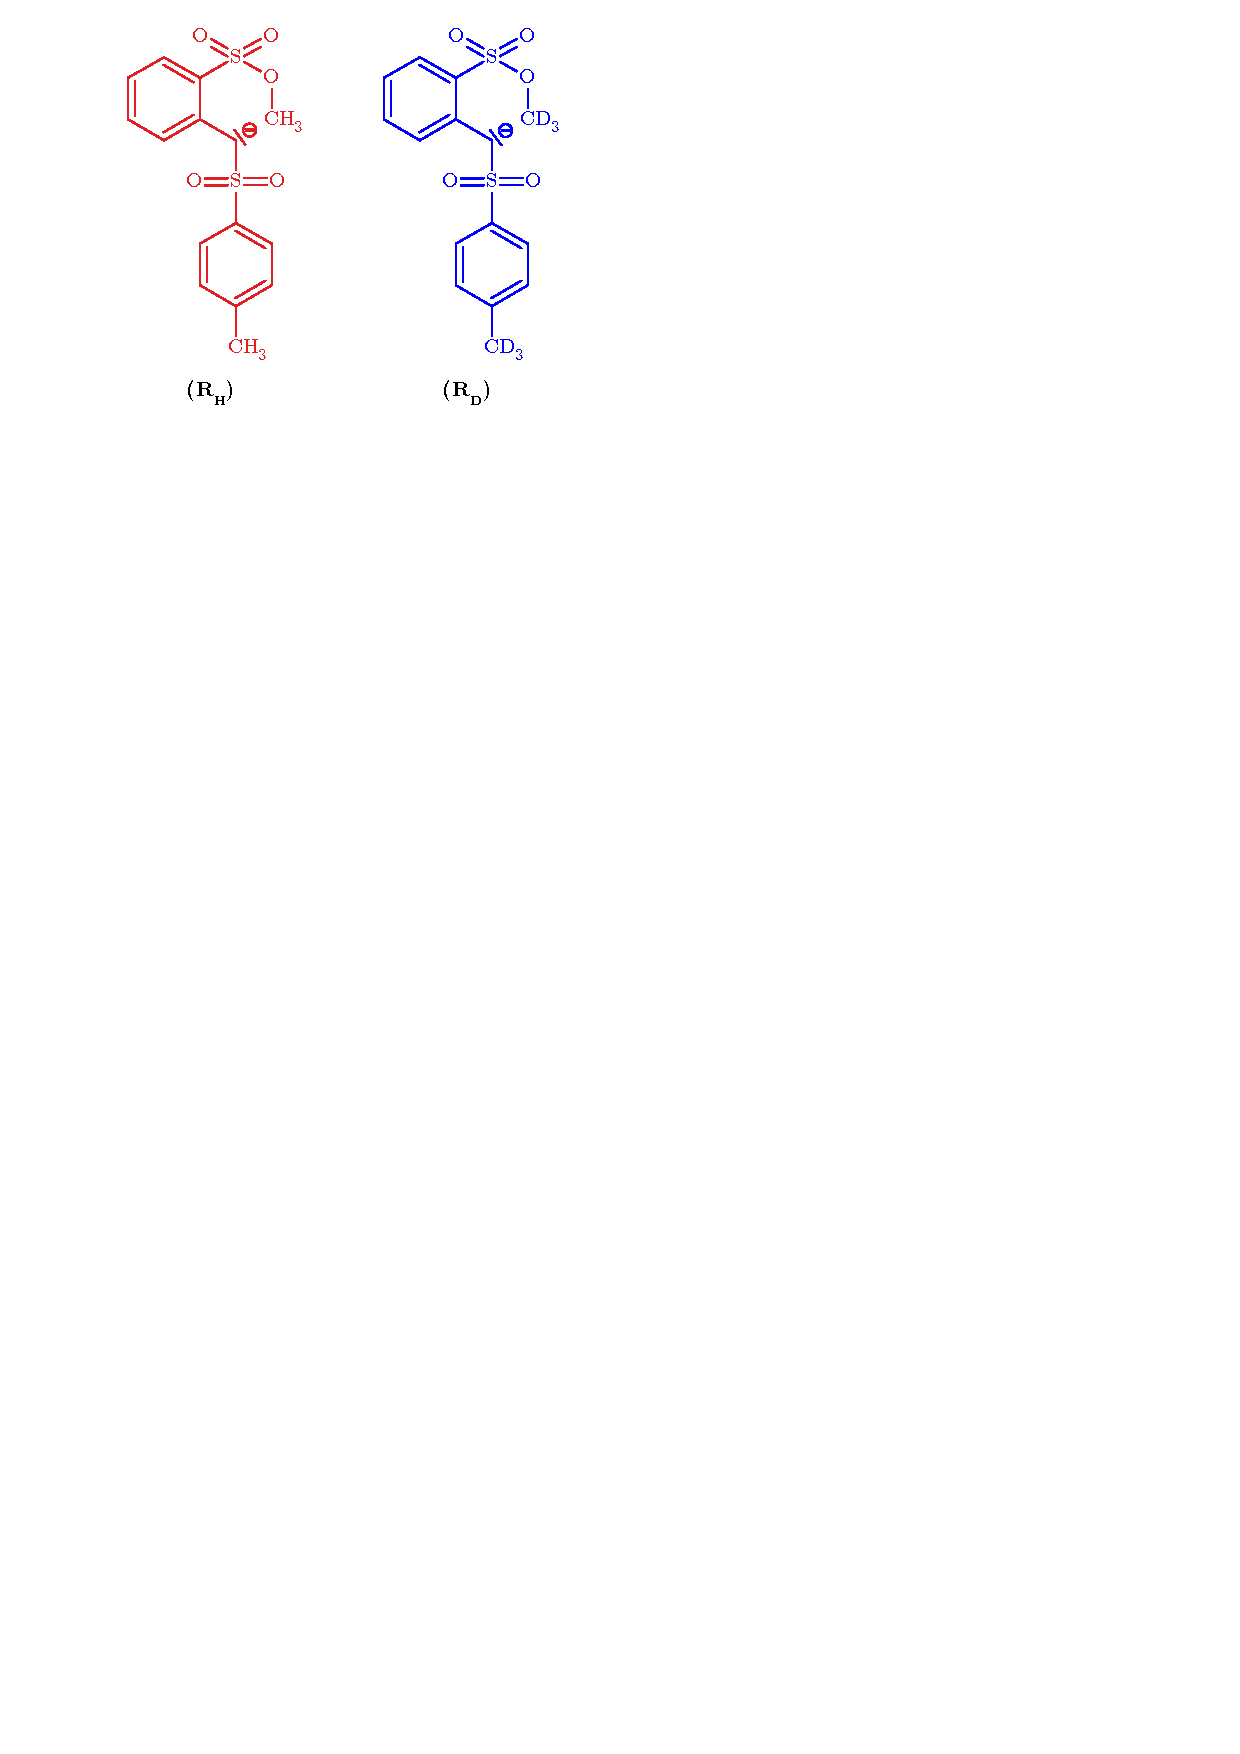
\includegraphics[scale=1.]{chimiePC/orga/eschenmoser.pdf}.
    \end{center}
    Ces molécules réagissent entre elles par substitution nucléophile.
\end{EnvUplevel}
\question Identifiez les groupes nucléophile et nucléofuge de la molécule et en déduire le mécanisme prédominant.

\question Identifiez les 6 réactions possibles et donnez leurs 4 produits formés. \\
On pourra utiliser la notation ---Bs--- (benzènesuflonyle) pour désigner \hspace{-1em} {\footnotesize\chemfig{\text{\color{white}M}-[,.9]*6(=-=(-S(=[3]O)(=[-3]O)-[,.9])-=-=-)}}.

\question \textsf{À l'oral :} Justifiez rapidement l'appellation $\mathrm{S_Ni}$ pour les mécanismes intramoléculaires.

\uplevel{Le résultat de l'expérience d'Eschenmoser est 4 produits trouvés en proportions quasi identiques \mbox{$1:1:1:1$}.}

\question Quelles réactions n'ont pas eu lieu ? Comment qualifier cette sélectivité ?

\uplevel{Nous allons voir pourquoi ces réactions n'ont pas eu lieu. Nous allons tout d'abord nous intéresser aux réactions intramoléculaires.}

\question En supposant que le cycle formé lors du mécanisme concerté est de  même géométrie qu'un cyclohexane en série aliphatique, représentez l'état de transition de la réaction intramoléculaire. \\
On pourra utiliser des notations abrévier les parties superflues des molécules.

\question Conclure quant à la sélectivité observée.

\plusloin A. Eschenmoser \emph{et al.} Endocyclische SN‐Reaktionen am gesättigten Kohlenstoff ?, \textit{Helvetica Chimica Acta}, Vol. 53, No. 8, \textbf{1970},  2059--2069.

\end{questions}
\end{exercise}